Notre billard est un peu bizarre car il est juste constitué de deux demi-droites de même origine, et notre bille est dans le secteur angulaire le "plus petit" formé par ces deux bandes. Ceci se représente comme suit.

\medskip

\begin{center}
	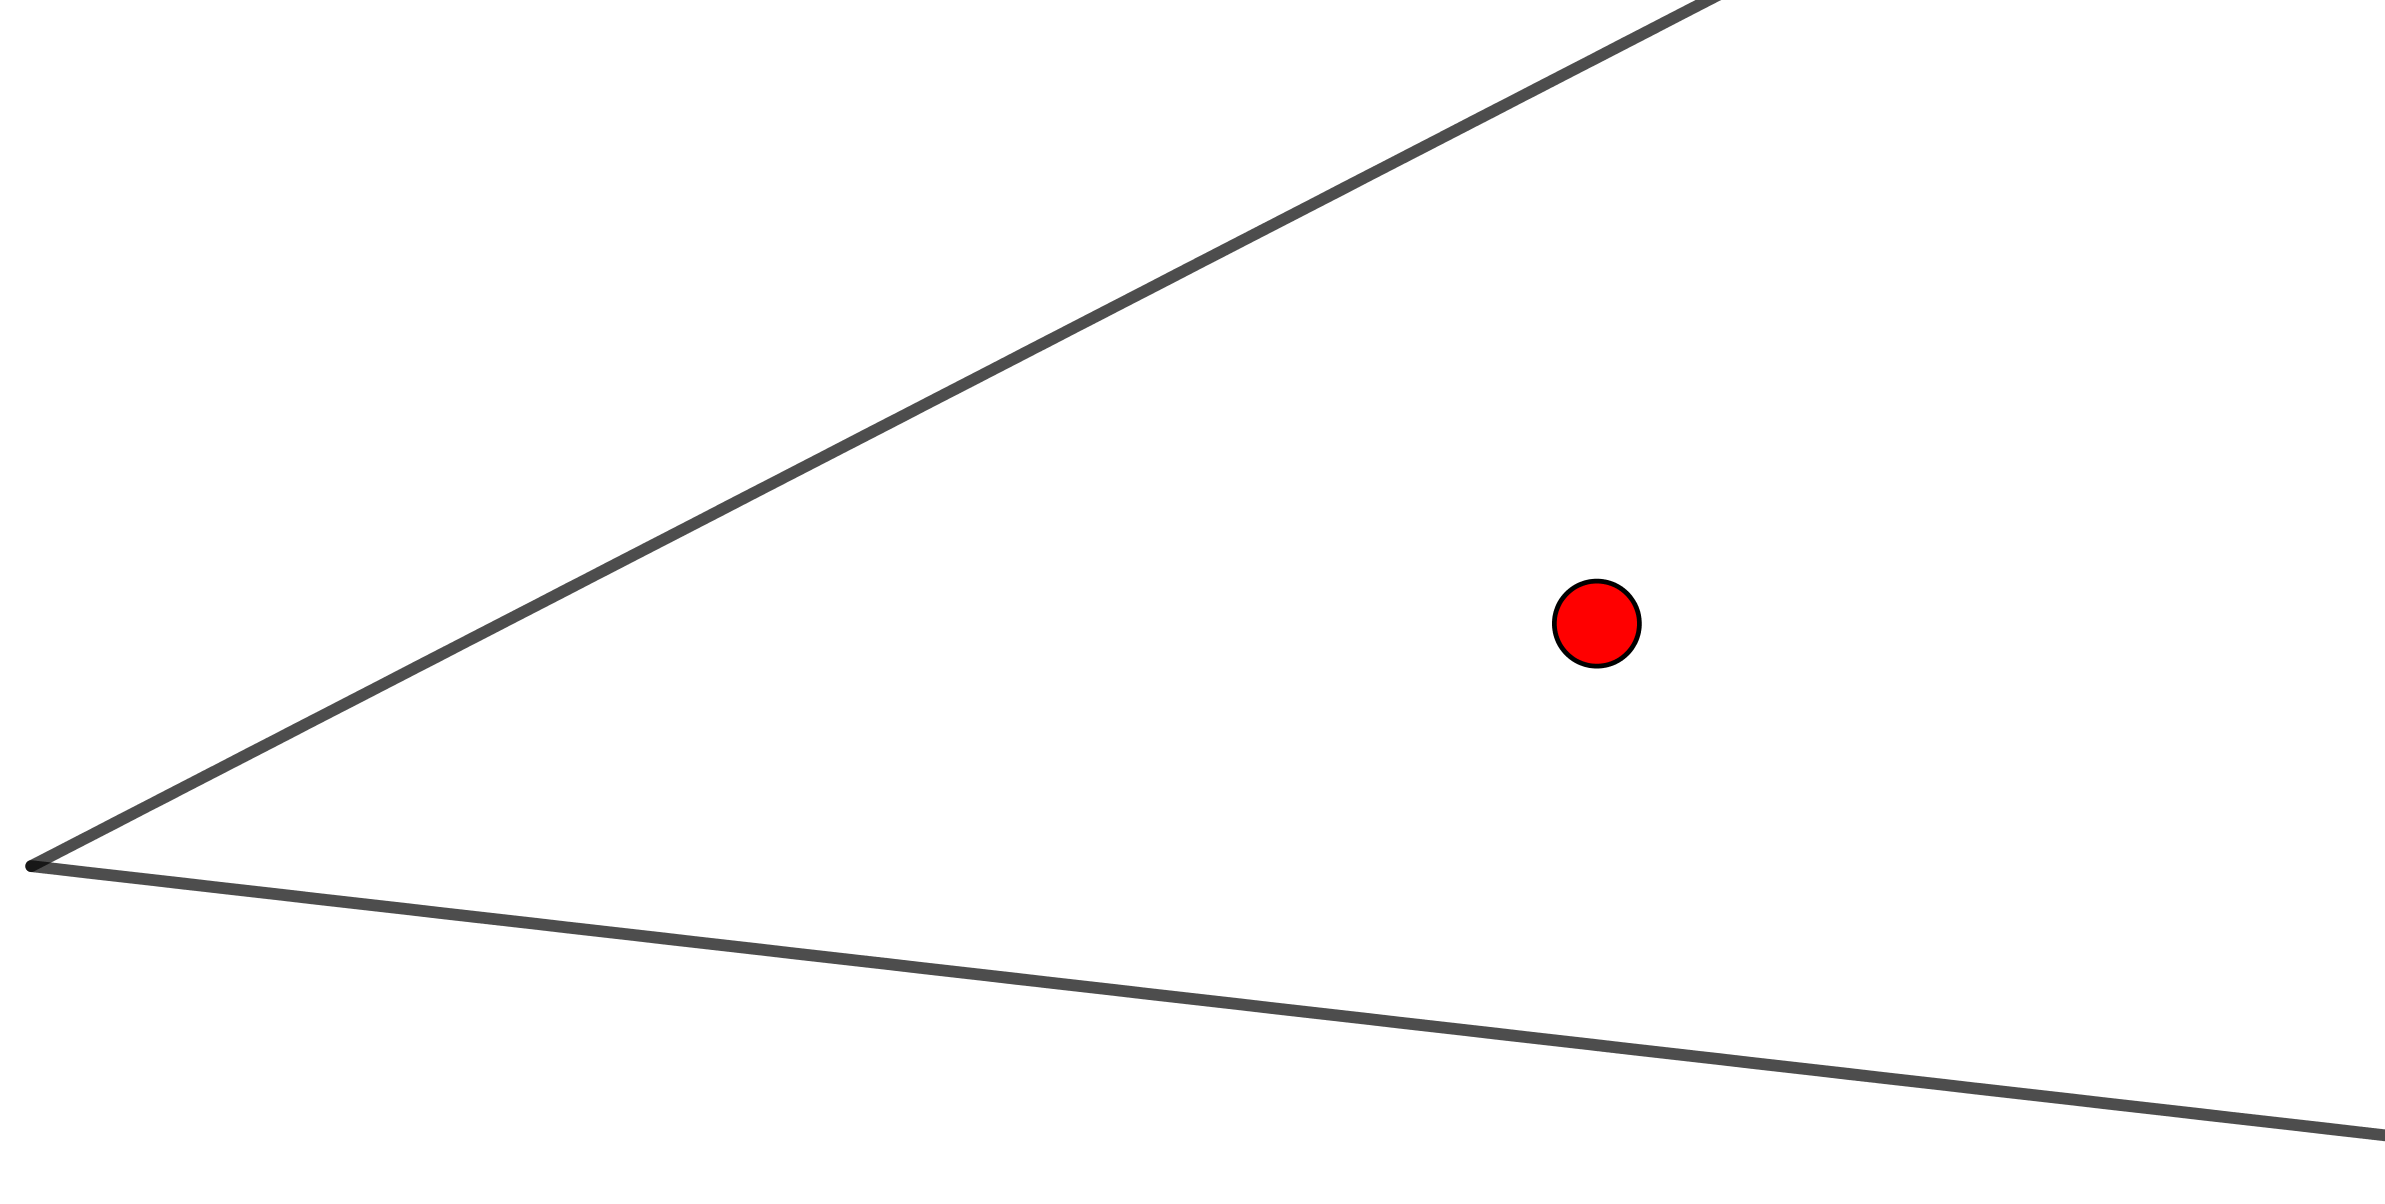
\includegraphics[width=12cm]{basic-math-pool/empty.png}
\end{center}

Dans la suite, nous considérons que notre bille est en fait un point, et du coup nous ne considérons pas les effets de rotation de la bille, et de plus nous ignorons les frottements, autorisant ainsi la bille à se balader vers l'infini et au-delà \emph{(tout ceci pour plus de réalisme)}.

\medskip

Concrètement, on pourrait se munir de deux miroirs plans verticaux et d'une source pouvant envoyer, dans un plan horizontal, un rayon laser dans une direction donnée.